\documentclass{article}
\textheight 23.5cm \textwidth 15.8cm
%\leftskip -1cm
\topmargin -1.5cm \oddsidemargin 0.3cm \evensidemargin -0.3cm
%\documentclass[final]{siamltex}

\usepackage{verbatim}
\usepackage{fancyhdr}
\usepackage{graphicx}

%\pagestyle{fancy} \lhead{FDM Homework Template} \chead{}
%\rhead{\bfseries Yan XU}
%
%\lfoot{} \cfoot{} \rfoot{\thepage}
%\renewcommand{\headrulewidth}{0.4pt}
%\renewcommand{\footrulewidth}{0.4pt}
%

%利用TEX排版系统的CTEX中文套装
\usepackage[UTF8,noindent]{ctex}
%等式对齐
\usepackage{amsmath}
\usepackage{amssymb}

\title{极小曲面和网格参数化}
\author{陈柯}

\begin{document}
	\maketitle
	
	\section{实验目的}
	
	1.	实现极小曲面生成
	
	2.  实现网格参数化,2种权重和2种边界
	
	\section{方法}
	1. 极小曲面:只要令边界点不动,每个内部点的微分坐标变为0,即
	$$\delta_i=v_i-\sum_{j}\omega_jv_j=0$$
	这里$v_j$为里$v_i$的邻结点,$\omega_j$为均匀权重。
	
	2.网格参数化:把边界点固定到二维的正方形边界或圆边界上,每个内部点的微分坐标变为0,
	即$$\delta_i=v_i-\sum_{j}\omega_jv_j=0$$
	这里$v_j$为里$v_i$的邻结点,$\omega_j$为均匀权重或Cotangent权重。
	
	3.权重的种类:(还要均一化)
	
	均匀权重:$\omega_j=1$
	
	Cotangent权重:$\omega_j=\cot{\alpha}+\cot{\beta}$
	\clearpage
	\section{结果}
	首先我实现了极小曲面的接口,以下是效果:
	\begin{figure}[htbp]
		\centering
		\begin{minipage}{0.49\linewidth}
			\centering
			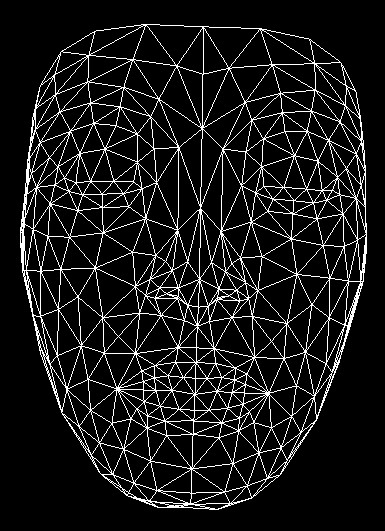
\includegraphics[width=0.9\linewidth]{init.JPG}
			\caption{原三角网格}
		\end{minipage}
		%\qquad
		\begin{minipage}{0.49\linewidth}
			\centering
			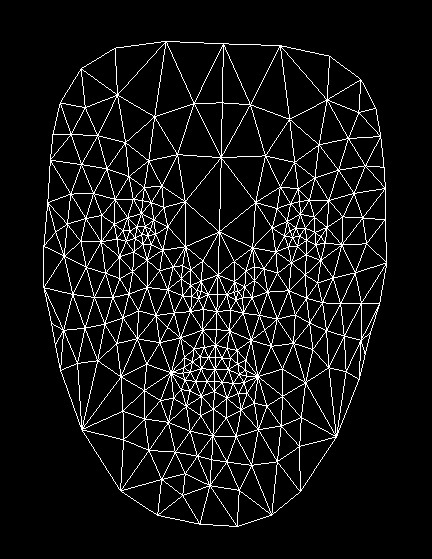
\includegraphics[width=0.9\linewidth]{mini.JPG}
			\caption{极小化后的网格}
		\end{minipage}
	\end{figure}
\clearpage
	然后是参数化,我这里采用了组合框控件实现了4种参数化,如下图:
	\begin{figure}[htb]
		\caption{参数化组合框} \centering
		\begin{center}
			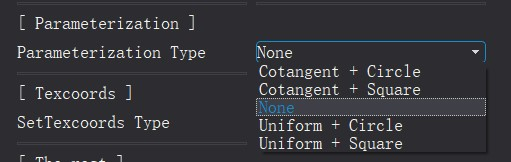
\includegraphics[width=2in]{combobox.jpg}
		\end{center}
	\end{figure}

	以下是4种参数化的效果(用的也是和极小曲面一样的人脸网格):
	\begin{figure}[htbp]
		\centering
		\begin{minipage}{0.49\linewidth}
			\centering
			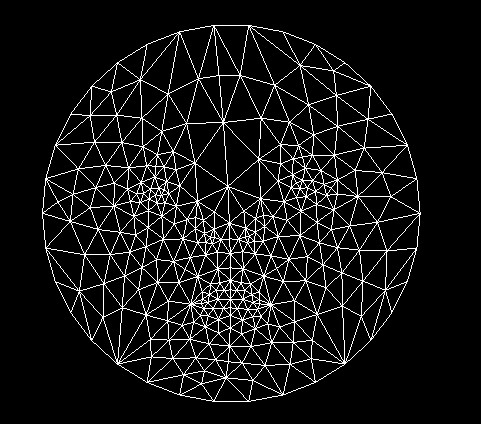
\includegraphics[width=0.8\linewidth]{UC.JPG}
			\caption{均匀权重+固定到圆形边界}
		\end{minipage}
		%\qquad
		\begin{minipage}{0.49\linewidth}
			\centering
			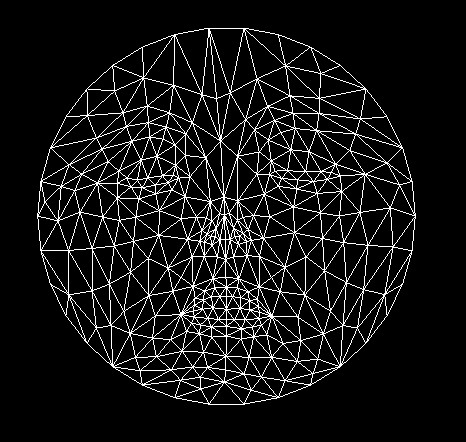
\includegraphics[width=0.8\linewidth]{CC.JPG}
			\caption{Cotangent权重+固定到圆形边界}
		\end{minipage}
	\end{figure}

	\begin{figure}[htbp]
		\centering
		\begin{minipage}{0.49\linewidth}
			\centering
			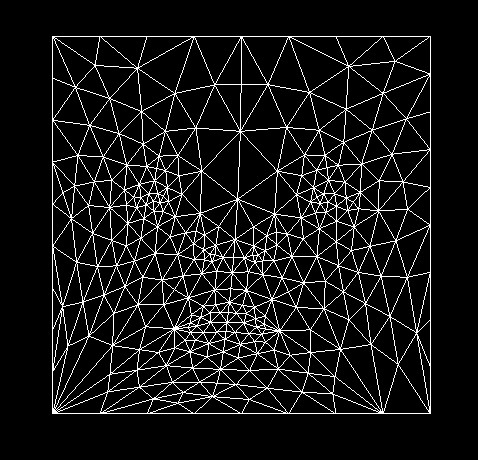
\includegraphics[width=0.7\linewidth]{US.JPG}
			\caption{均匀权重+固定到正方形边界}
		\end{minipage}
		%\qquad
		\begin{minipage}{0.49\linewidth}
			\centering
			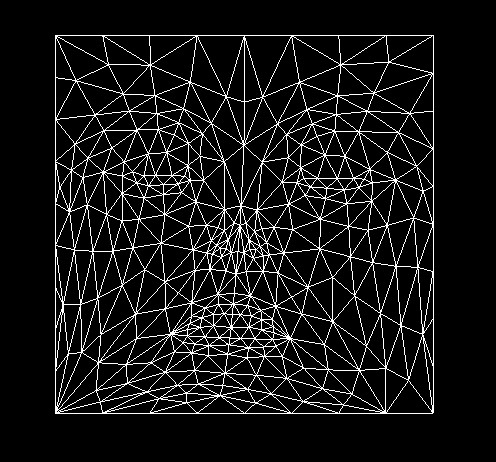
\includegraphics[width=0.7\linewidth]{CS.JPG}
			\caption{Cotangent权重+固定到正方形边界}
		\end{minipage}
	\end{figure}
	由于Cotangent权重一定程度上保留了原网格的几何性质,所以参数化后的网格更像原网格,或
	者说眼睛和嘴巴等部分看起来更自然。
	\clearpage
	最后我用组合框控件实现了4种参数化的纹理坐标,如下图:
	\begin{figure}[htb]
		\caption{\label{table.label} 纹理坐标组合框} \centering
		\begin{center}
			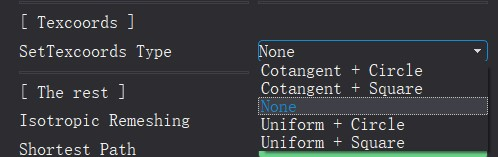
\includegraphics[width=2in]{texcoords.jpg}
			\label{figure.label}
		\end{center}
	\end{figure}
	选好了纹理坐标后,我们就可以上传图片实现网格的纹理贴图:
	\begin{figure}[htbp]
		\centering
		\begin{minipage}{0.49\linewidth}
			\centering
			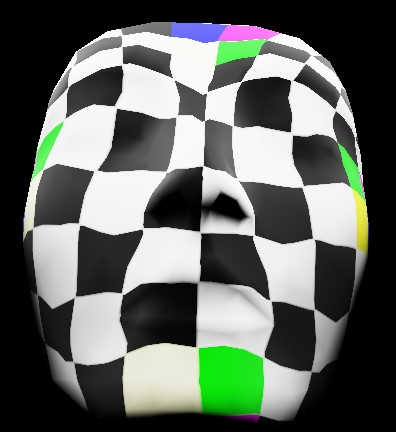
\includegraphics[width=0.6\linewidth]{UCtex.JPG}
			\caption{均匀权重+固定到圆形边界}
		\end{minipage}
		%\qquad
		\begin{minipage}{0.49\linewidth}
			\centering
			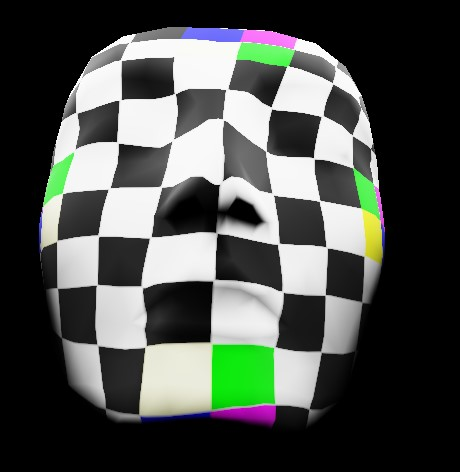
\includegraphics[width=0.7\linewidth]{CCtex.JPG}
			\caption{Cotangent权重+固定到圆形边界}
		\end{minipage}
	\end{figure}

	\begin{figure}[htbp]
		\centering
		\begin{minipage}{0.49\linewidth}
			\centering
			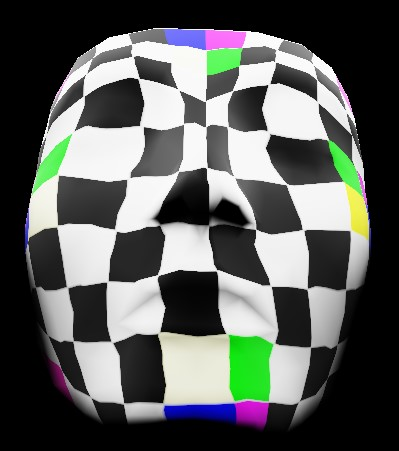
\includegraphics[width=0.6\linewidth]{UStex.JPG}
			\caption{均匀权重+固定到正方形边界}
		\end{minipage}
		%\qquad
		\begin{minipage}{0.49\linewidth}
			\centering
			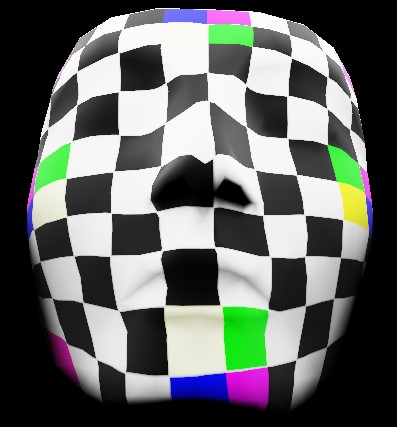
\includegraphics[width=0.7\linewidth]{CStex.JPG}
			\caption{Cotangent权重+固定到正方形边界}
		\end{minipage}
	\end{figure}
	从纹理贴图中也能看出Cotangent权重效果更好,线条的扭曲没有均匀权重严重。
\section{参考文献}
  $[1]$Michael S. Floater, Parametrization and smooth approximation of surface 
  triangulations ,Computer Aided Geometric Design 14 (1997) 231-250 
\end{document}
